\chapter{CEMicro Implementation}
\label{sec:impl}

In this chapter, we dive into the practical implementation of CEMicro. The microservice consists of three layers, the frontend, the backend, and the database. Each layer is treated in some detail. Though the information is very technical, I made an effort to keep it simple enough for less technical affine readers to understand. In no way does this chapter cover the implementation comprehensively but provides an overview of the most critical decisions.


\section{Setting up the Development Environment}

\begin{itemize}
  \item \done{Visual Studio Code (code editor) https://code.visualstudio.com/}
  \item \done{Git (version control) https://git-scm.com/}
  \item \done{Virtualisation with Docker}
  \item \done{Node.js}
  \item \done{Challenge: Setting up git/bash on windows}
  \item \done{Challenge: File permissions for docker on windows}
\end{itemize}

It seems trivial to treat the development environment in this chapter, but that would be a disservice to any programmer. The development environment is an essential part of writing an application and can be as much of a time sink as software bugs, as we will see. I am used to developing on a Mac operating system. Mac is based on Unix and offers a built-in Bash shell, basically just like any Linux machine, while Windows uses an entirely different foundation for its operating system. All the technologies which work with cloud computing and distributed services operate on Linux systems because the internet runs on Linux\footnote{Yeah, sorry Microsoft}. We are talking about technologies like Git version control, Docker container virtualization, and Node.js and its packet manager NPM. The machine Capgemini provided me with is a Windows computer.

I first set up Visual Studio Code, currently the most popular code editor, especially among web developers and developed by Microsoft ~\cite{stackoverflow.2019}. Next, I set up git\footnote{https://git-scm.com/downloads}, which comes with a complete Bash environment, howbeit with a reduced feature set. Bash stands for ``Bourne Again Shell'' and is a variation of the default Unix shell, a command-line interface. An average user usually never uses the command line but interacts with generated user interfaces (GUI) of a program. In a shell, the user can interact with programs by typing one-line commands. For example, \inlinecode{rm -rf test-dir/} instructs the simple ``remove'' program to delete the ``test-dir'' folder with all its content. This way of using programs is handy for programmers and system administrators in their work, especially if running commands on remote computers through SSH\footnote{Secure Shell, a way to use the shell of a remote computer} sessions.

\begin{figure}[ht]
  \centering
  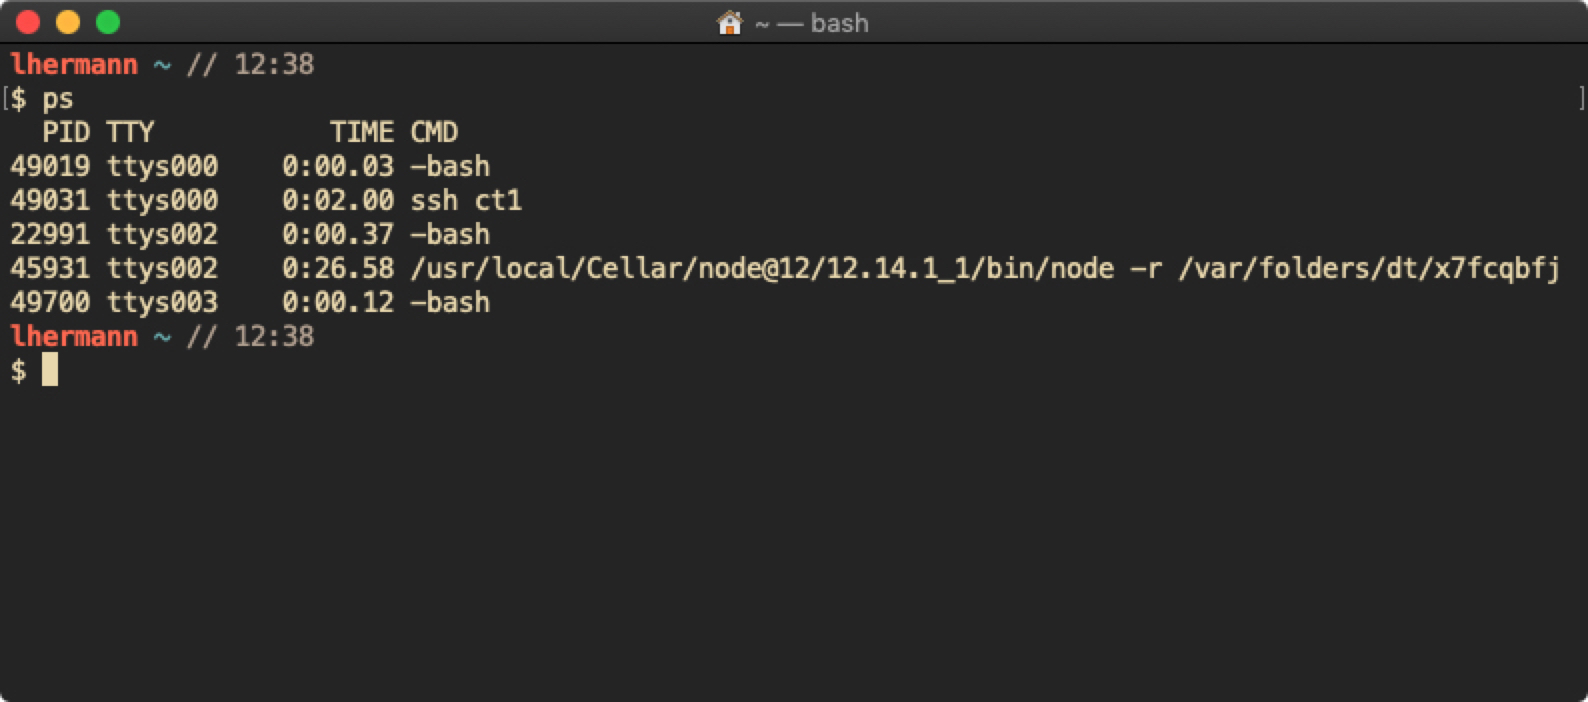
\includegraphics[width=0.75\linewidth]{assets/example-bash-window.jpg}
  \caption{Example for a bash terminal executing the 'ps' command}
\end{figure}

Because I planned to write the entire application in JavaScript, I set up a Node.js environment\footnote{https://nodejs.org/}. JavaScript is an interpreted language; it means that the code does not need to compile to machine code like Java, for example, but the Node runtime reads the JavaScript file and translates it for the computer on the fly. It means that I can start a program by simply typing \inlinecode{node main.js} into the shell, which then executes the contents of main.js. Furthermore, I can install a JavaScript tool like Nodemon\footnote{https://www.npmjs.com/package/nodemon} with \inlinecode{npm install nodemon} that watches the JS\footnote{JS is short for JavaScript} files on my systems and restarts the application whenever I change the file. This provides instant feedback, in the form of an updated application or error messages, and makes development comfortable.

\begin{figure}[ht]
  \centering
  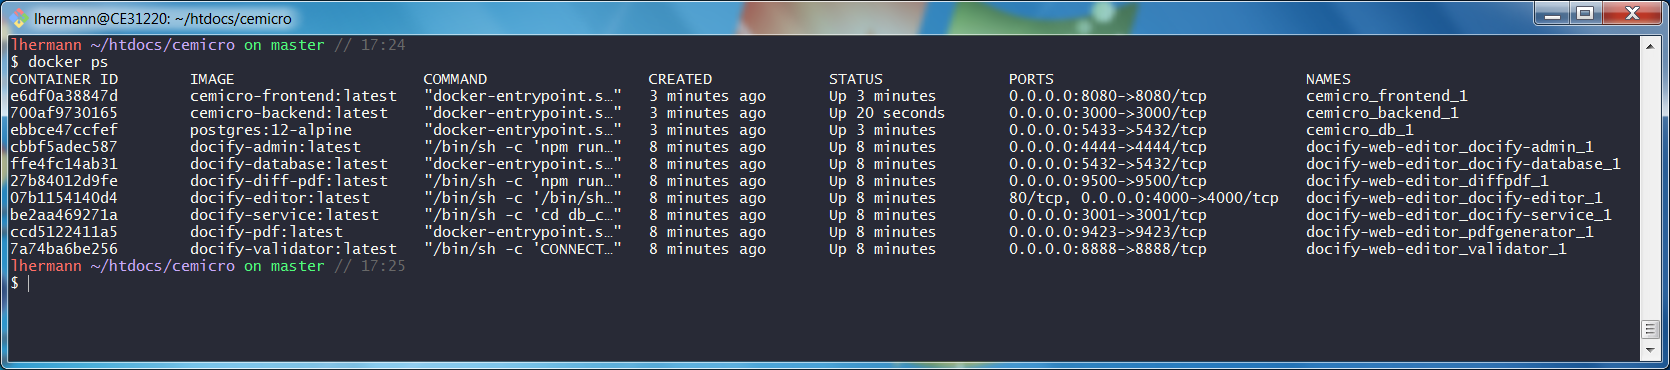
\includegraphics[width=1\linewidth]{assets/terminal-docker-ps.png}
  \caption{'docker ps' shows all running docker containers}
\end{figure}

Docker\footnote{https://www.docker.com} is a tool that can run the software in a container. A container is like an application that brings its entire ecosystem with it, howbeit a very simplified one, so that it doesn't become too large. This application then runs in isolation from anything else on the host system. This is very useful because it allows the developer to run dependencies like databases or other services for an application without the hassle of installing them on the system manually and the difficulty of handling different versions. For the development of CEMicro, I ran my PostgreSQL database in a docker container. I also needed a running instance of the Docify service, itself a combination of six containers, which I downloaded and started in Docker. The \inlinecode{docker-compose} command provides a very convenient way to start all required containers for an entire application at once. These containers then run in the background, and the developer can concentrate on his current code.

One challenge I faced with setting up bash on windows was the limited way in which the shell environment of the git application works. Familiar commands and shell setups on Unix machines were not available under the Windows environment, and it took me a while to work around this limitation. Another problem arose with Docker in that it works with Unix file system permissions. On a Unix system, every file has a set of nine permissions, read, write and execute separate for the user, the group and others\footnote{The details about Unix file permissions go beyond this chapter, for more info see https://www.tutorialspoint.com/unix/unix-file-permission.htm}, this system is part of the hard drive format and OS kernel\footnote{A kernel is the bottom-most layer of an operating system}. Windows does not have any file system permissions; it's not part of the operating system. Instead, Windows handles users and groups with dedicated services, and this is also the reason why there are so many more worms and viruses for Windows. The Docker environment for Windows fakes those permissions. But for specific requirements, for example, when using Docker volumes, these permissions need to be changed to work. It is possible to do this, but I couldn't find out how and I assume it has to do with a user management service, which is not accessible under the closed business setup of the machine Capgemini gave me. It, therefore, took me a while to find a workaround for Docker volumes so that they only exist within the virtual environment and don't come in contact with the Windows host.

\section{Application Programming Interface}
\label{sec:impl:api}

\begin{itemize}
  \item \done{REST}
  \item \done{Swagger/OpenApi}
  \item \done{Single source of truth}
  \item \done{Discarded: Saving Templates in CEMicro (see single source of truth page)}
  \item \done{Discarded: swagger-tools}
\end{itemize}

The CEMicro service deals with three different objects\footnote{In programming, an object is like a container for data.} — the template, the configurable element, and its items. The template contains the template string in combination with sample data for the placeholders inside the template. The configurable element, as discussed in the section on page \pageref{sec:arch:understanding}, a holder for the individual properties as well as the name and the default value. And the configurable element item which is one individual set of the properties of table \ref{table:ce-properties}.

\begin{table}[!ht]
  \begin{center}
    \begin{tabular}{|l|l|p{6cm}|}
      \hline
      Action & Route & Description \\
      \hline\hline
      GET & /templates & Get a list of template abstracts \\
      \hline
      GET & /templates/\{market\} & Get a list of template abstracts by market \\
      \hline
      GET & /templates/\{market\}/\{name\} & Get a template by market and name \\
      \hline
      GET & /templates/\{market\}/\{name\}/pdf & Get the PDF of a template by market and name \\
      \hline
      GET & /configurable-elements & Get a list of Elements for the given parameters \\
      \hline
      GET & /configurable-elements/\{id\} & Get an Elements by id \\
      \hline
      PATCH & /configurable-elements/\{id\} & Update an Element by id \\
      \hline
      GET & /configurable-elements/\{id\}/items & Get all Items for an Element \\
      \hline
      POST & /configurable-elements/\{id\}/items & Create an Item for an Element \\
      \hline
      GET & /configurable-element-items/\{id\} & Get an ElementItem by id \\
      \hline
      PUT & /configurable-element-items/\{id\} & Update an ElementItem by id \\
      \hline
      PATCH & /configurable-element-items/\{id\} & Patch an ElementItem by id \\
      \hline
      DELETE & /configurable-element-items/\{id\} & Delete an ElementItem by id \\
      \hline
    \end{tabular}
  \end{center}
  \caption{API endpoints of the CEMicro backend}
  \label{table:api-endpoints}
\end{table}

Table \ref{table:api-endpoints} shows all the API endpoints of CEMicro. We can see that a market-name tuple uniquely identifies a template. That means a template name itself is not unique because two markets, like the Netherlands and France, can use the same template name. To make sure these templates do not get mixed up, they are namespaced by the market. Also, observe that there is no POST or PUT actions for templates, that's because templates are not saved in the CEMicro database but fetched from the Docify service whenever requesting this endpoint.

One important concept is the single source of truth, meaning that one piece of information only exists in one place. This is especially important when working with microservices and other concepts of distributed architectures. Since the services and thus the programming logic is distributed, information, by necessity, also needs to be distributed. However, as just established, we do not want duplication of information. Thus, with microservice architectures, one piece of information should only exist inside a single microservice. CEMicro solves this the single source of truth principle by requesting templates on the fly from the Docify service and only saving configurable elements and their items in its database.

Initially, I planned to include templates in the database because it is such an essential part of the application. The frontend needs to list all the available templates, and configurable elements are essentially placeholders within the template. However, saving the templates in our database would mean duplication of the information because Docify handles them. It would be possible for docify to send a notification to CEMicro whenever a template changes, but the easier way is to fetch templates fresh every time we need them.

Both elements and element items are saved in the CEMicro database and entirely managed by it. It is common to provide CRUD actions for every resource. CRUD stands for CREATE-READ-UPDATE-DELETE, the four principal actions for data. In the table, we can see that element items have all four CRUD operations plus PATCH, which is a partial update function where only a subset of properties has to be provided. Configurable elements, however, do not have four CRUD operations. That's because I decided to create them on the fly. Whenever the user opens a template in the frontend, it requests all the elements from the backend. At that point, the backend parses the template string for a list of all the necessary configurable elements. It then compares this list with the database and creates an element that is missing before returning the complete list of elements to the frontend. This way, the user is saved the hassle of manually creating an element after adding it to the template in Docify. It saved one working step. However, during the debriefing with the project manager, we concluded that it would be better to additionally offer the manual option to the user so he can create and delete elements as needed.

\begin{figure}[ht]
  \centering
  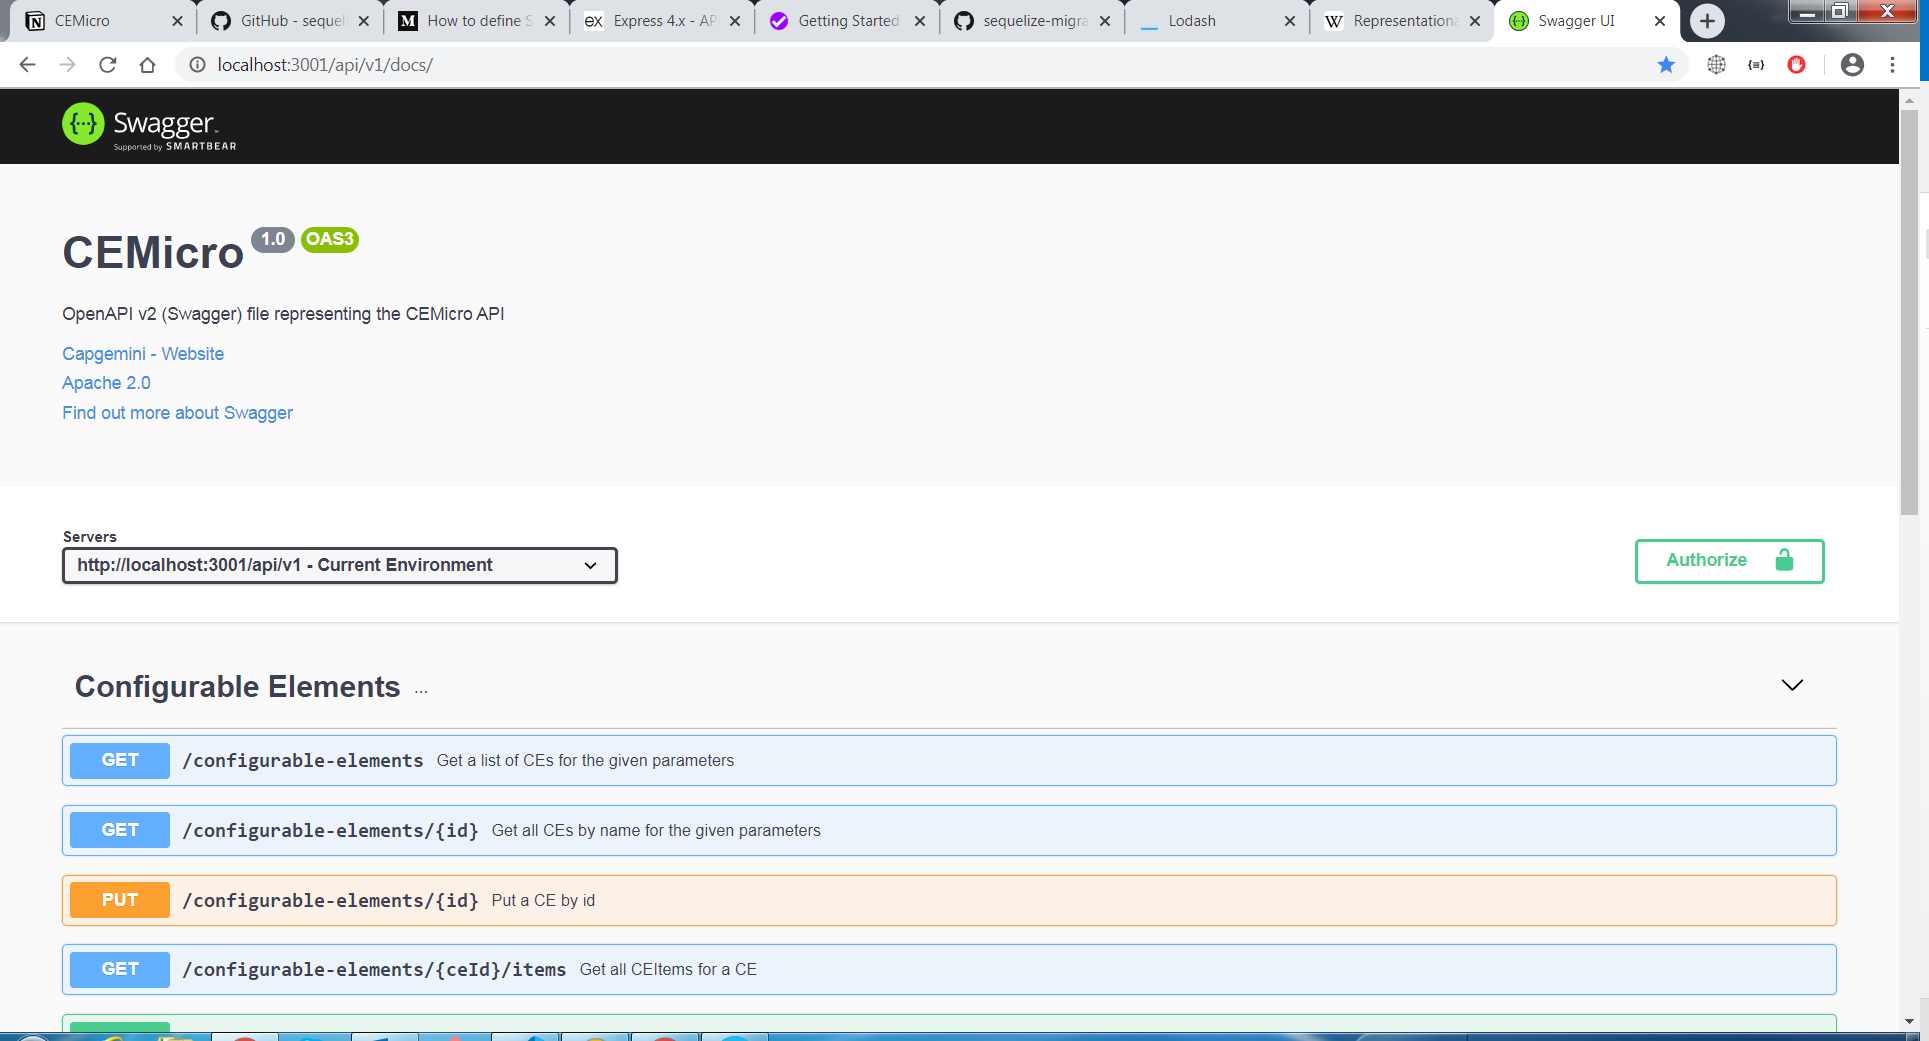
\includegraphics[width=0.8\linewidth]{assets/swagger-api-docs.png}
  \caption{Interactive API documentation with Swagger}
  \label{fig:api-docs}
\end{figure}

The appendix \ref{sec:appendix:openapi} shows an excerpt of the \inlinecode{openapi.yml} file. This file is the authoritative documentation for the API. Swagger\footnote{https://swagger.io}, the open-source project behind the OpenAPI standard, provides tools to generate an interactive documentation page from this file automatically, see figure \ref{fig:api-docs}. Docify uses a library called ``swagger-tools'' to automatically generate some scaffolding for their code directly from their OpenAPI file. This approach saves some repetitive coding and helps to tie the functional code and the documentation together. For CEMicro, however, I decided to omit this library and add everything by hand because the project is stale, it didn't see any updates for two years, and does not support the latest version of the OpenAPI specification\footnote{See https://www.npmjs.com/package/swagger-tools}.


\section{Backend Framework with Express.js}

\begin{itemize}
  \item \done{Tool: Express}
  \item \done{Tool: Express Validator}
  \item \done{MVC -> MVCS (Model View Controller Service)}
\end{itemize}

I tried to mostly include libraries that the Docify team already used to make the transition more manageable, and so that the two microservices can merge with little friction if desired. Fortunately, Docify tended to use the bread and butter libraries for JavaScript servers: Express ~\cite{stateofjs.2019}. Express\footnote{https://expressjs.com} is a minimalist Node.js framework that takes care of HTTP requests and routing with no additional frills. Besides, Express leaves a free choice of the file structure.

\begin{figure}[ht]
  \centering
  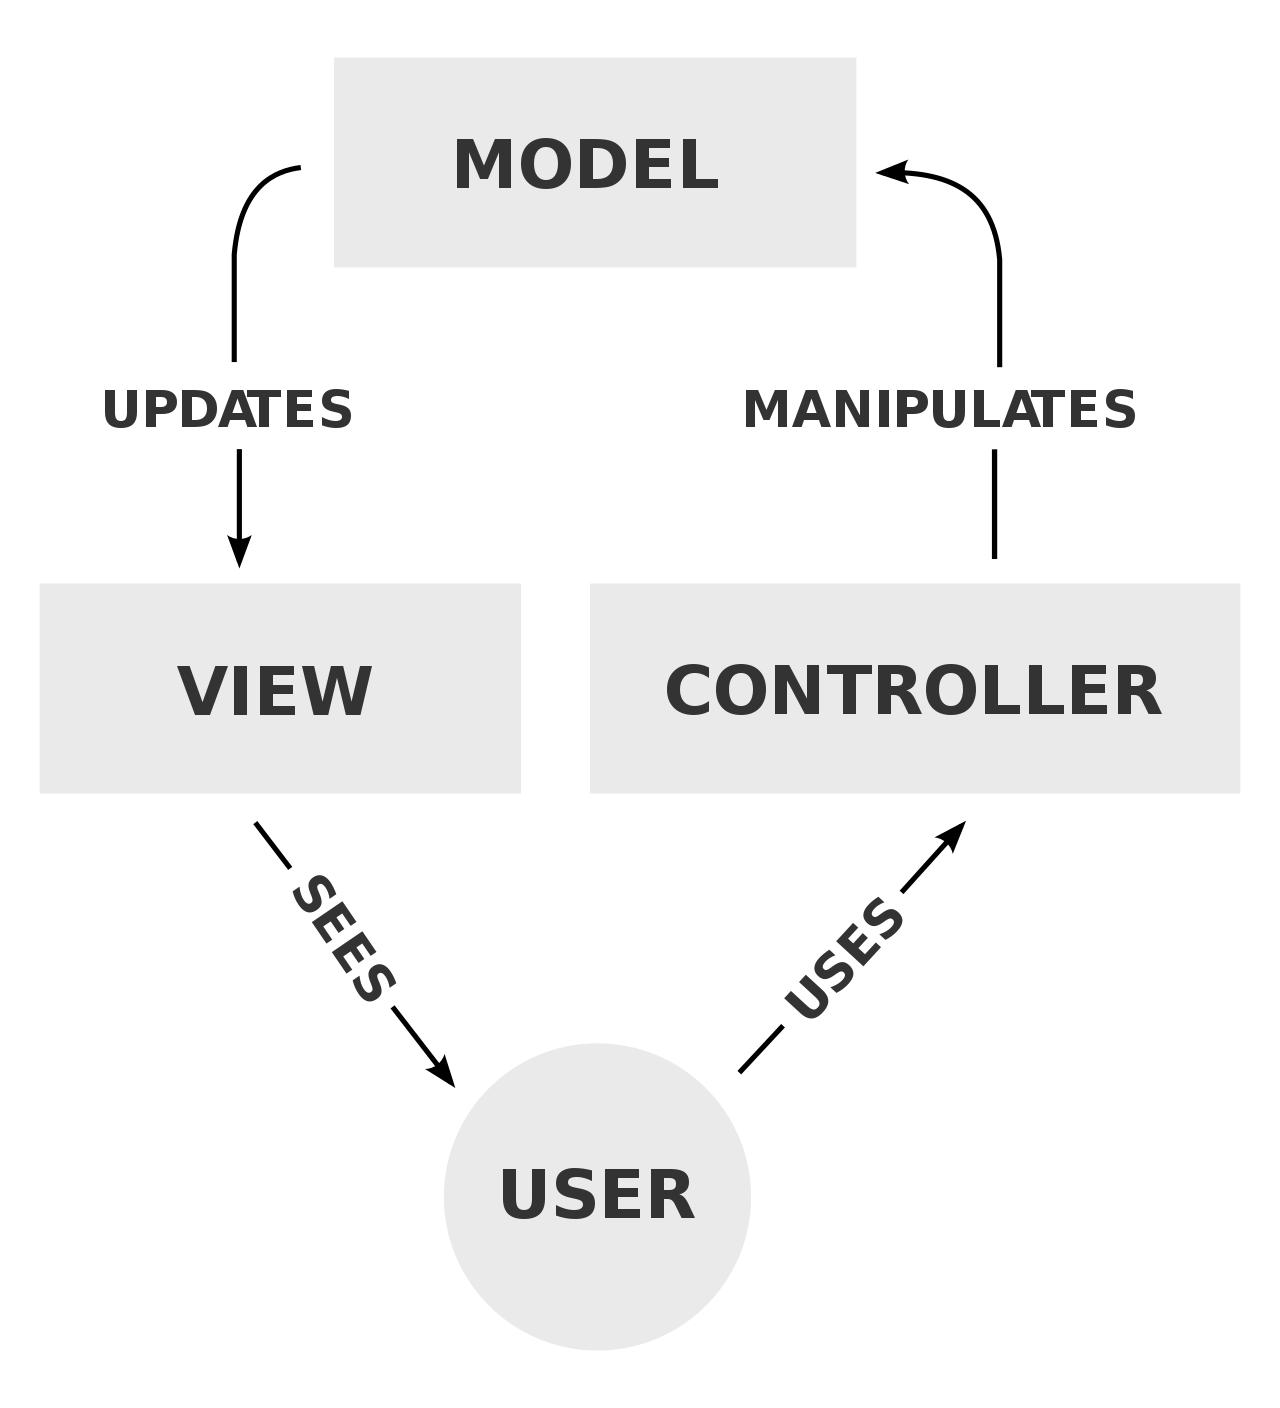
\includegraphics[width=0.3\linewidth]{assets/mvc-process.png}
  \caption{Diagram of interactions within the MVC pattern}
  \source{https://en.wikipedia.org/wiki/Model–view–controller}
  \label{fig:mvc-process}
\end{figure}

In backend development, it has become common to use the Model-View-Controller (MVC) architecture. User interactions go to the controller, a function that decides which data models to load and what view to show to the user. A view is a general word for a page of an application. In pure API backends, that is, backends that don't render a view but only provide an API, the view layer is usually omitted. The controller directly returns the data to the caller of the API.

Additionally, a service layer is often used between the controller and the model. The controller calls the service to get the data it needs. The service is responsible for the core business logic, loading the data from the database by calling the model, and then performing the necessary data manipulations. Appendix \ref{sec:appendix:mvcs} shows a code example for the controller, service, and model of the element component. Sequelize\footnote{https://sequelize.org/v5/}, an ORM\footnote{Object-relational mapping, see https://en.wikipedia.org/wiki/Object-relational_mapping} library for Node.js, handles the data model and database access; see the next section.

There are three additional preliminary concerns for every server-side application. The first is data validation for which I used the express-validator\footnote{https://express-validator.github.io/docs/} library. It takes care that the parameters provided by the user can be processed and don't contain any malicious code. The second concern is user access management, which we decided to omit because of the brevity of the provided time. We also decided to omit the third concern, which is testing. Omitting tests is considered a developer sin, but because CEMicro is more a proof of concept, we felt comfortable in saving the development time.

\section{Data persistance with PosgreSQL}

\begin{itemize}
  \item \done{Sequelize https://github.com/sequelize/express-example}
  \item \done{Discarded: Flyway-db, Umzug}
  \item \done{Migrations: Sequelize}
\end{itemize}

All the decisions for which data goes where were made at this point, which makes the database implementation trivial. As mentioned in Section \ref{sec:arch:technology} I decided on PostgreSQL. Setting up the database itself at this point means starting a Docker container with the official PostgreSQL Docker image\footnote{https://hub.docker.com/_/postgres/}. The challenge with databases lies in keeping the schemata up to date with the data model of the backend. For programming code, git version control keeps track of all changes and can handles conflicts when two developers edit the same lines of a file simultaneously. With git, every programmer can always pull the current version of the code from a central repository. Such a system doesn't exist for databases. Instead, developers write migrations, a set of instructions to bring the database schema from an older to a newer state. These migrations are committed to version control so that developers can update their local database as needed. I looked at several migration solutions for Node.js.

The Docify team recommended Flyway\footnote{https://flywaydb.org} to me, but it is primarily for Java applications, and I couldn't find a suitable package for Node.js. Another recommendation I found was Umzug\footnote{https://www.npmjs.com/package/umzug}, a well-supported package, but it doesn't handle the actual database manipulation. The documentation for Umzug recommended the Sequelize ORM\footnote{https://sequelize.org/v5/} to interface with the database. After looking at Sequilize, I realized that it provides a database-agnostic ORM, which means that I can write database access in its custom format, and Sequilizes translates it into valid SQL statements for PostgreSQL. Not only that, Sequelize makes it trivial to change the database dialect, for example, from PostgreSQL to MySQL, with a simple configuration option, and it takes care of the rest. And Sequelize comes with its system for database migrations, which I decided to use.


\section{Frontend Framework with Vue.js}

Originally the plan was to write the frontend in Angular\footnote{https://angular.io}. Angular is a client-side framework created by Google and popular among more traditional software companies for its Java-like approach in the directory structure and use of the static type JavaScript language extension Typescript. I agreed with this decision, primarily because the Docify team also used it. I am mentioning the Docify team repeatedly here for the mere reason that it is the only other service inside the POS team written with modern web-development principles. It is the only other microservice inside POS in existence. However, Angular turned out to have a rather steep learning curve and is overly complicated for such a small application as CEMicro. After completing several tutorials, I understood why 35\% of frontend engineers say they used Angular and would never use it again\footnote{See figure \ref{fig:frontend-framework-usage}}. Having said that, I realized I already mentioned this in the previous chapter, but it bears repeating.

Going with vue turned out to be a breeze. I already had ample experience with the framework and knew which plugins to include for the required use cases. Because CEMicro is a proof of concept, my mentor and I felt justified with the decision. I set up the frontend in such a way as to include the most commonly used techniques so that a rewrite into Angular by another team, later on, would be frictionless. For example, I exclusively used Bootstrap\footnote{https://getbootstrap.com} components for the user interface. Bootstrap is the go-to CSS framework for standard user interfaces like the admin page of CEMicro. Having a working user interface build on these principles as an example, the next team can rewrite it quickly if necessary.

I also made sure the frontend looks almost identical to Docify so it can be merged if desired and so that users already familiar with the Docify interface can use CEMicro intuitively.

\begin{figure}[ht]
  \begin{subfigure}[b]{0.5\linewidth}
    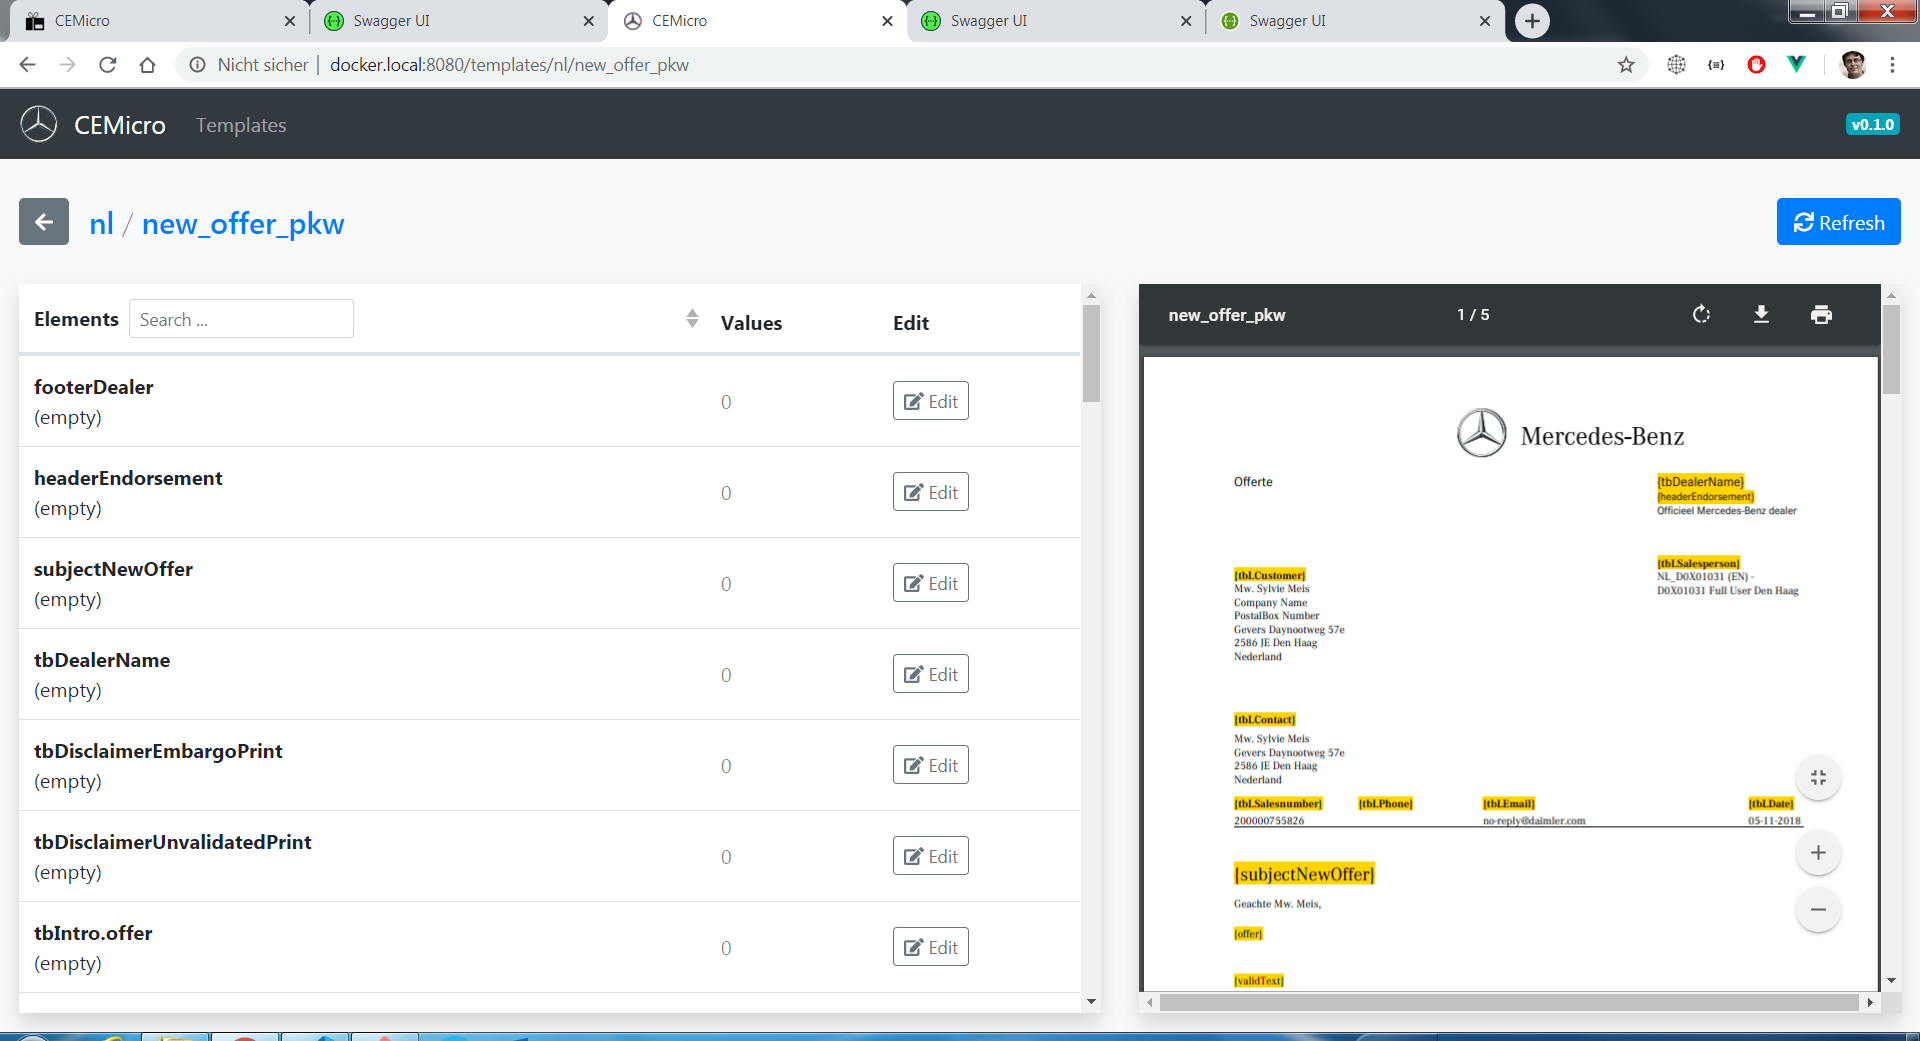
\includegraphics[width=\linewidth]{assets/cemicro-element-list.png}
    \caption{CEMicro element editor}
  \end{subfigure}
  \begin{subfigure}[b]{0.5\linewidth}
    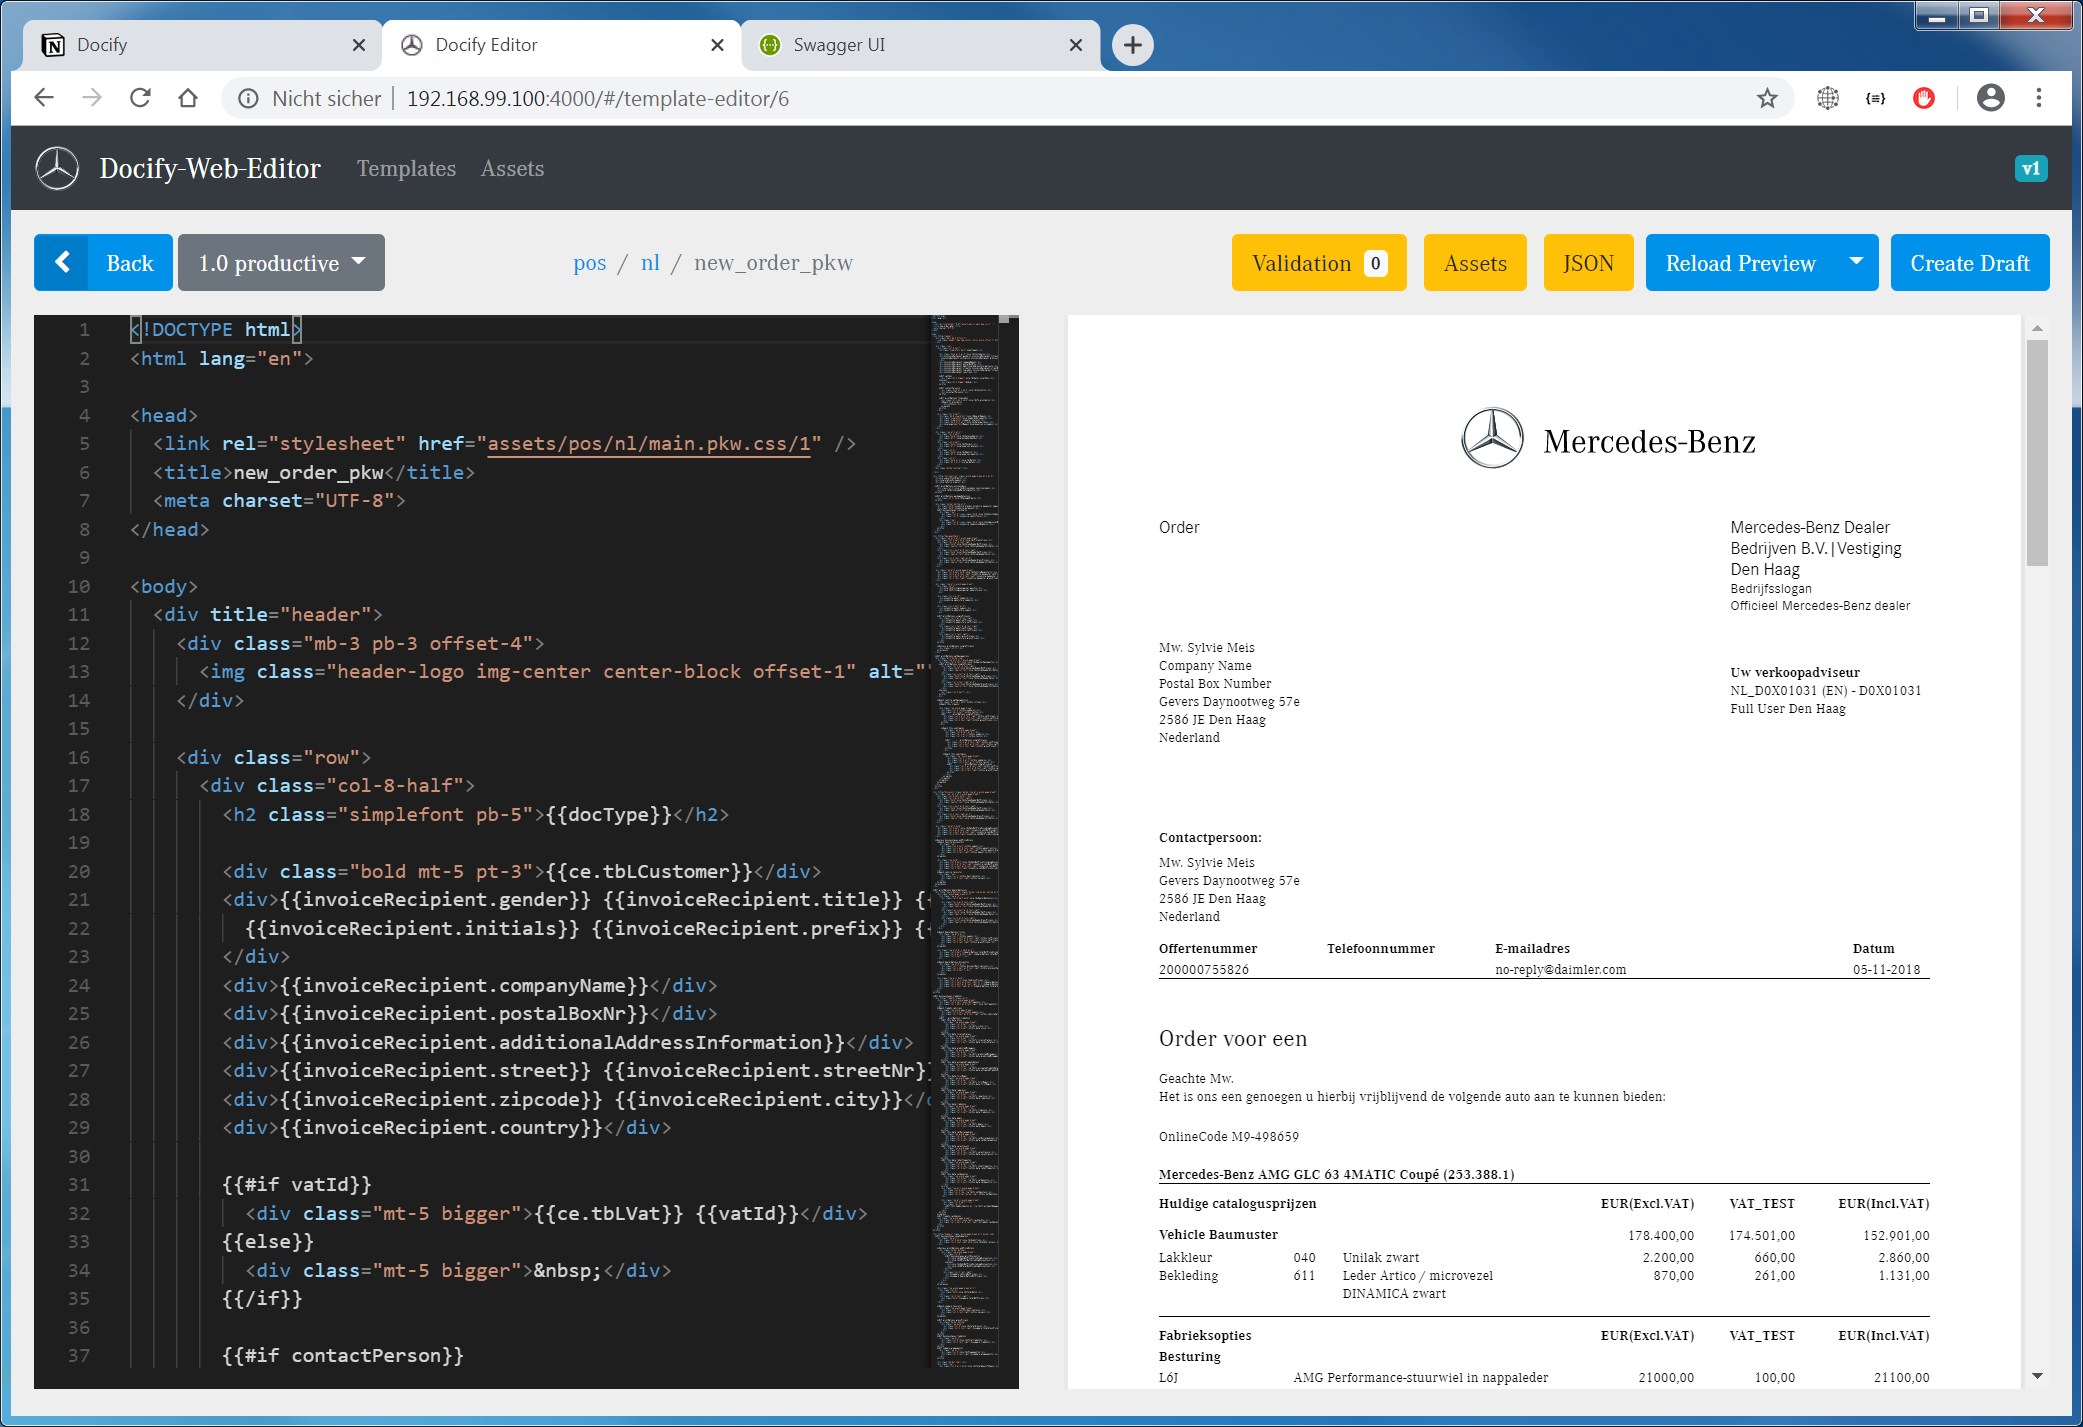
\includegraphics[width=\linewidth]{assets/docify-editor.png}
    \caption{Docify template editor}
  \end{subfigure}
  \caption{CEMicro's user interface is similar to that of Docify}
  \label{fig:cemicro-docify-ui}
\end{figure}


\section{Virtualisation with Docker}

\begin{itemize}
  \item \done{install packages, build, prune packages}
\end{itemize}

If an application is packaged with Docker, then starting the application on a new machine is a breeze. PostgreSQL uses an official predefined Docker image, which works with minimal configuration, in this case, only a few environment variables. Both the backend and frontend use the official Node.js image. Only the image is not enough in this case because the programming code has to go into the container as well. One way to do that is with so-called volumes. A volume is a directory existing on the local machine and in the docker container at the same time. This arrangement is beneficial when using Docker during development but not for running it in production. I didn't use Docker during development because it tends to be a little slow. After all, the Docker volume has to sync the filesystem between the host and its virtual machine. Instead, I am running the application right on my system with my Node.js runtime, which is significantly faster. But for the production build, I want to have everything inside the container. To achieve this, we add a Dockerfile to the application, using the Node.js image as a foundation and building upon it with our code.

For example, here is the Dockerfile for the backend:

\begin{lstlisting}
FROM node:12-alpine

WORKDIR /var/app

COPY --chown=node:node . .

RUN npm install --production

ENV SERVICE_HOST=192.168.99.100
ENV SERVICE_PORT=3000
ENV NODE_ENV=production
ENV DB_HOST=db
ENV DB_USER=cemicro
ENV DB_PASS=123456
ENV DB_PORT=5432

EXPOSE 3000

USER node

CMD ./node_modules/.bin/sequelize db:migrate && npm run production
\end{lstlisting}

We can see that it uses the \inlinecode{node:12-alpine} image as a foundation, copies the files from the backend into the new image, and installs all NPM dependencies. It then defines some environment variables and instructs the container to run a set of commands when on start. An ``image'' in Docker language is like a blueprint, and a ``container'' takes that blueprint and creates a live instance from it. Multiple containers can be created from one image.

The backend is particularly simple because it doesn't require any build step; the code is just copied and executed directly. The frontend, however, posed an interesting challenge because a build step is required. The frontend is made up of special \inlinecode{.vue} component files which cannot be executed directly. First, we have to transform them into valid HTML, CSS, and JavaScript files during a build process. But to keep the image as small as possible, all the code that was only required for the build needs to be removed before finishing the Docker image. It turns out that NPm provides a command to ``prune'' development code from the filesystem after the build, here is the relevant excerpt of the frontend Dockerfile:

\begin{lstlisting}
RUN npm install
RUN npm run build
RUN npm prune --production
\end{lstlisting}

And with that, the containerization of the CEMicro application is complete. Now the single command \inlinecode{docker-compose up} takes care of building and starting all three parts of the application, including running the migrations for a new database, and it is then usable through the browser.


\section{Interfacing with the monolith development team}

\begin{itemize}
  \item \done{Changes to Docify}
\end{itemize}

Interfacing with the rest of the team was probably my most significant challenge in this task. Robin, my mentor, went to great length to make sure I had everything I needed and was taken care of. But even his endeavors can only go so far. In the end, I was part of my CEMicro team of one, only talking now and then with others from POS when necessary. This situation, of course, is particular to my position as a bachelor student with a project that only lasts four months, and yet, some lessons can be learned from it.

When extracting a microservice, as with any other software development, make sure there is a regular exchange of all the key parties involved. Don't only bring in the main stakeholder at the end of the project, as was the case with my project. Chances are once the boundaries are specified and understood, the team would want to simplify concepts that grew in complexity over the years. Take this chance, simplifying software is always a worthwhile endeavor.

Next, don't treat your microservice as not relevant. If your company wants to move forward, embrace change like this and take it seriously. I assume the problem was that Capgemini doesn't own the POS project itself but is doing client work for Mercedes Benz. It means the primary stakeholder is another layer removed from the actual developer. Instead of Mercedes wanting to invest in a service-oriented architecture, I had the impression that Capgemini tried to entice its client to do so. This situation was certainly not the most fertile ground for such technological innovation, especially since it doesn't translate into hard coin right away.

In the end, I did work with the team responsible for Docify. I tried to understand their application and their pain points. For example, Docify has two different user interfaces, one for administration and the other for daily use. Both users interfaced use their dedicated backend service. However, these two services use the same database. I asked about this arrangement, and they made it clear that this arrangement was the wrong choice and that these sub-services were cut too small. I also contributed to their codebase by adding a small API endpoint, which I needed for CEMicro. Beyond this, however, I worked alone.


\section{Documentation of CEMicro}

\begin{itemize}
  \item \done{Providing a foundation for others to build on (Confluence, Readme, Thesis)}
\end{itemize}

Documentation is a point not particular to microservices but probably of more importance here. Any application needs proper documentation, so new developers can hit the ground running. When using a microservice architecture, it is even more likely that programmers need to make changes that have never worked on the service before. This thesis is one way of documenting CEMicro and should work as a reference for others. More important, however, is to leave proper breadcrumbs where others would expect them.

Confluence is a kind of wiki page developed by Atlassian, the company behind Jira, which Capgemini uses for its project management. It is the place where the entry point for everything POS can be found, so it is the place where I added at least an introduction to CEMicro.

The other place is the \inlinecode{README.md} file in the root directory of the application code. The \inlinecode{README.md} became a de-facto convention among developers to look for basic usage instruction of a program. CEMicro's README offers simple first steps to start the application with Docker and to set it up for development.


\section{Wrap-up}

In the end, most implementation decisions are practical and situational. I used technology I am familiar with, checked libraries the Docify project used and made sure that they have proper documentation and active development. The end goal is to make it easy for oneself and others to understand the code and pick up development where I left off. Using well-supported libraries and writing robust documentation are the two ways to help software live longer. Finally, communication is crucial but also one of the harder aspects of software development.



